%%%%%%%%%%%%%%%%%%%%%%%%%%%%%%%%%%%%%%%%%
% Beamer Presentation
% LaTeX Template
% Version 2.0 (March 8, 2022)
%
% This template originates from:
% https://www.LaTeXTemplates.com
%
% Author:
% Vel (vel@latextemplates.com)
%
% License:
% CC BY-NC-SA 4.0 (https://creativecommons.org/licenses/by-nc-sa/4.0/)
%
%%%%%%%%%%%%%%%%%%%%%%%%%%%%%%%%%%%%%%%%%

%----------------------------------------------------------------------------------------
%	PACKAGES AND OTHER DOCUMENT CONFIGURATIONS
%----------------------------------------------------------------------------------------

\documentclass[
	11pt, % Set the default font size, options include: 8pt, 9pt, 10pt, 11pt, 12pt, 14pt, 17pt, 20pt
	%t, % Uncomment to vertically align all slide content to the top of the slide, rather than the default centered
	%aspectratio=169, % Uncomment to set the aspect ratio to a 16:9 ratio which matches the aspect ratio of 1080p and 4K screens and projectors
]{beamer}

\graphicspath{{Images/}{./}} % Specifies where to look for included images (trailing slash required)

\usepackage{booktabs} % Allows the use of \toprule, \midrule and \bottomrule for better rules in tables

%----------------------------------------------------------------------------------------
%	SELECT LAYOUT THEME
%----------------------------------------------------------------------------------------

% Beamer comes with a number of default layout themes which change the colors and layouts of slides. Below is a list of all themes available, uncomment each in turn to see what they look like.

%\usetheme{default}
% \usetheme{AnnArbor}
% \usetheme{Antibes}
% \usetheme{Bergen}
% \usetheme{Berkeley}
% \usetheme{Berlin}
% \usetheme{Boadilla}          %%
% \usetheme{CambridgeUS}       
% \usetheme{Copenhagen}
% \usetheme{Darmstadt}
% \usetheme{Dresden}
% \usetheme{Frankfurt}
% \usetheme{Goettingen}         
% \usetheme{Hannover}
% \usetheme{Ilmenau}
% \usetheme{JuanLesPins}
% \usetheme{Luebeck}
\usetheme{Madrid}
% \usetheme{Malmoe}
% \usetheme{Marburg}
% \usetheme{Montpellier}       %%
% \usetheme{PaloAlto}            %%
% \usetheme{Pittsburgh}
% \usetheme{Rochester}
% \usetheme{Singapore}
% \usetheme{Szeged}
% \usetheme{Warsaw}
\usepackage[flushleft]{threeparttable}
%----------------------------------------------------------------------------------------
%	SELECT COLOR THEME
%----------------------------------------------------------------------------------------

% Beamer comes with a number of color themes that can be applied to any layout theme to change its colors. Uncomment each of these in turn to see how they change the colors of your selected layout theme.

% \usecolortheme{albatross}
% \usecolortheme{beaver}
% \usecolortheme{beetle}
% \usecolortheme{crane}
% \usecolortheme{dolphin}
% \usecolortheme{dove}
% \usecolortheme{fly}
% \usecolortheme{lily}
% \usecolortheme{monarca}
% \usecolortheme{seagull}
% \usecolortheme{seahorse}
\usecolortheme{spruce}
% \usecolortheme{whale}
% \usecolortheme{wolverine}

%----------------------------------------------------------------------------------------
%	SELECT FONT THEME & FONTS
%----------------------------------------------------------------------------------------

% Beamer comes with several font themes to easily change the fonts used in various parts of the presentation. Review the comments beside each one to decide if you would like to use it. Note that additional options can be specified for several of these font themes, consult the beamer documentation for more information.

\usefonttheme{default} % Typeset using the default sans serif font
%\usefonttheme{serif} % Typeset using the default serif font (make sure a sans font isn't being set as the default font if you use this option!)
%\usefonttheme{structurebold} % Typeset important structure text (titles, headlines, footlines, sidebar, etc) in bold
%\usefonttheme{structureitalicserif} % Typeset important structure text (titles, headlines, footlines, sidebar, etc) in italic serif
%\usefonttheme{structuresmallcapsserif} % Typeset important structure text (titles, headlines, footlines, sidebar, etc) in small caps serif

%------------------------------------------------

%\usepackage{mathptmx} % Use the Times font for serif text
\usepackage{palatino} % Use the Palatino font for serif text

%\usepackage{helvet} % Use the Helvetica font for sans serif text
% \usepackage[default]{opensans} % Use the Open Sans font for sans serif text
%\usepackage[default]{FiraSans} % Use the Fira Sans font for sans serif text
%\usepackage[default]{lato} % Use the Lato font for sans serif text

%----------------------------------------------------------------------------------------
%	SELECT INNER THEME
%----------------------------------------------------------------------------------------

% Inner themes change the styling of internal slide elements, for example: bullet points, blocks, bibliography entries, title pages, theorems, etc. Uncomment each theme in turn to see what changes it makes to your presentation.

% \useinnertheme{default}
\useinnertheme{circles}
% \useinnertheme{rectangles}
% \useinnertheme{rounded}
% \useinnertheme{inmargin}

%----------------------------------------------------------------------------------------
%	SELECT OUTER THEME
%----------------------------------------------------------------------------------------

% Outer themes change the overall layout of slides, such as: header and footer lines, sidebars and slide titles. Uncomment each theme in turn to see what changes it makes to your presentation.

% \useoutertheme{default}
% \useoutertheme{infolines}
% \useoutertheme{miniframes}
% \useoutertheme{smoothbars}
%\useoutertheme{sidebar}
% \useoutertheme{split}
% \useoutertheme{shadow}
% \useoutertheme{tree}
% \useoutertheme{smoothtree}

% \setbeamertemplate{footline} % Uncomment this line to remove the footer line in all slides
%\setbeamertemplate{footline}[page number] % Uncomment this line to replace the footer line in all slides with a simple slide count

%\setbeamertemplate{navigation symbols}{} % Uncomment this line to remove the navigation symbols from the bottom of all slides

%----------------------------------------------------------------------------------------
%	PRESENTATION INFORMATION
%----------------------------------------------------------------------------------------

\title[Semidefinite Programming]{Semidefinite Programming} % The short title in the optional parameter appears at the bottom of every slide, the full title in the main parameter is only on the title page

\subtitle{Applications in approximating NP-Complete problems \& Matrix Completetion} % Presentation subtitle, remove this command if a subtitle isn't required

\author[]{Dimitri Lopez \and Xinshi Wang \and Jenny Gao} % Presenter name(s), the optional parameter can contain a shortened version to appear on the bottom of every slide, while the main parameter will appear on the title slide

\institute[RPI]{Rensselaer Polytechnic Institute} % Your institution, the optional parameter can be used for the institution shorthand and will appear on the bottom of every slide after author names, while the required parameter is used on the title slide and can include your email address or additional information on separate lines

% \date[\today]{International Symposium of Explorers \\ \today} % Presentation date or conference/meeting name, the optional parameter can contain a shortened version to appear on the bottom of every slide, while the required parameter value is output to the title slide

%----------------------------------------------------------------------------------------

\begin{document}

%----------------------------------------------------------------------------------------
%	TITLE SLIDE
%----------------------------------------------------------------------------------------

\begin{frame}
	\titlepage % Output the title slide, automatically created using the text entered in the PRESENTATION INFORMATION block above
\end{frame}

%----------------------------------------------------------------------------------------
%	TABLE OF CONTENTS SLIDE
%----------------------------------------------------------------------------------------

% The table of contents outputs the sections and subsections that appear in your presentation, specified with the standard \section and \subsection commands. You may either display all sections and subsections on one slide with \tableofcontents, or display each section at a time on subsequent slides with \tableofcontents[pausesections]. The latter is useful if you want to step through each section and mention what you will discuss.

\begin{frame}
	\frametitle{Presentation Overview} % Slide title, remove this command for no title

	\tableofcontents % Output the table of contents (all sections on one slide)
	% \tableofcontents[pausesections] % Output the table of contents (break sections up across separate slides)
\end{frame}

%----------------------------------------------------------------------------------------
%	Semidefinite Programming
%----------------------------------------------------------------------------------------

\section{Motivation for Linear Programming}
\begin{frame}[label={sec:org0f20b1e}]{Motivation for Semidefinite Programming}
\begin{itemize}
\item Linear Programming is a common constrained optimization technique with uses in:
\begin{itemize}
\item Math
\item Computer Science
\item Economics
\item Buisness
\end{itemize}
\item Wide applicability combined with fast runtimes makes linear programming quite popular
\end{itemize}
\pause
\noindent\rule{\textwidth}{0.5pt}
\begin{itemize}
\item Semidefinite programming (SDP) expands upon the ideas of linear programming
\begin{itemize}
\item SDP problems are more general
\item Widely used in combinatorial optimzation problems
\item Many NP-Hard problems can be approximated well with SDP
\end{itemize}
\end{itemize}
\end{frame}

\section{Overview of Linear Programming}

\begin{frame}[label={sec:org7e6dba1}]{Motivation for a Linear Program}
\begin{itemize}
\item Suppose that we have control over a set of variables: \(\vec{x} = [x_1, x_2, \ldots, x_n]^\top\)
\end{itemize}
\pause
\begin{itemize}
\item Where for each of these \(n\) variables we have an associated coefficient \(\vec{c} = [c_1, c_2, \ldots, c_n]^\top\)
\end{itemize}
\pause
\begin{itemize}
\item In the end we want to find the optimal value for the following equation:
\end{itemize}
\[
\min \vec{c} \cdot \vec{x}
\]
\end{frame}
\begin{frame}[label={sec:orgc3775a6}]{Motivation for a Linear Program}
\vspace{-3.5em}
\begin{gather*}
\min \vec{c} \cdot \vec{x} \\
\end{gather*}

\vspace{-1em}
\begin{itemize}
\item The problem is quite easy as is. What if each of these \(n\) variables
corresponds to how much of a given product that we want to buy?
\begin{itemize}
\item This would add additional constraints to what values \(\vec{x}\) could
take on.
\end{itemize}
\end{itemize}
\pause
\begin{itemize}
\item Each variable must satisfy some constraint, we can express this as:
\end{itemize}
\vspace{-2em}
\begin{align*}
\vec{a}_1 \cdot \vec{x} &\geq b_1 \\
\vec{a}_2 \cdot \vec{x} &\geq b_2 \\
& \vdots  \\
\vec{a}_n \cdot \vec{x} &\geq b_n \\
\end{align*}
\vspace{-3.5em}
\pause
\begin{itemize}
\item We can gather this into a single expression using a matrix
\end{itemize}
\[
\mathbf{A} \vec{x} \geq \vec{b}
\]

\pause
\vspace{-2em}
\begin{itemize}
\item Furthermore we often constraint \(\vec{x}\) to be non-negative: \(\vec{x} \geq
  0\).
\end{itemize}
\end{frame}

% \begin{frame}[label={sec:org14df325}]{Graphical Representation of Linear Inequalities}
% \begin{itemize}
% \item Graphically, the \(n\) constraints each create a \emph{half-space}
% \begin{itemize}
% \item Each half-space shows the viable region for \(\vec{x}\) given the
% constraint.
% \end{itemize}
% \item The intersection of the half-spaces is the set of possible solutions given by
% the white space below - also known as the feasible region
% \end{itemize}
% \begin{center}
% \includegraphics[width=.9\linewidth]{./.org-imgs/presentation.org_20230417-154715-fo5yDY.png}
% \end{center}

% \begin{itemize}
% \item Our goal is to find the value of \(\vec{x}\) that optimizes \(\min \vec{c}
%   \cdot \vec{x}\) and is within the feasible region
% \end{itemize}
% \end{frame}

\begin{frame}[label={sec:orgc3bccc9}]{Standard Form for a Linear Program}
\begin{align*}
  \begin{array}{ll@{}ll}
    \text{minimize}   & \vec{c} \cdot \vec{x}& \\
    \text{subject to} & \mathbf{A} \vec{x} &\geq  \vec{b} \\
                      & \vec{x} &\geq 0 \\
    \end{array}
\end{align*}
\pause
\begin{itemize}
\item Where \(\vec{x}\) are the variables that we have control over
\begin{itemize}
\item Example: Each variable of \(\vec{x}\) represents how much of a certain
product to purchase
\end{itemize}
\pause
\item \(\vec{c}\) is a set of corresponding coefficients for the variables of \(\vec{x}\)
\begin{itemize}
\item Example: Each variable of \(\vec{c}\) corresponds to how much each product costs
\end{itemize}
\pause
\item \(\min \vec{c} \cdot \vec{x}\) is the function we are trying to optimize
\begin{itemize}
\item Example: We want to minimize the cost of buying our products
\end{itemize}
\pause
\item \(\mathbf{A} \vec{x} \geq \vec{b}\) constraints on our solutions. Defines the
feasible region.
\begin{itemize}
\item Example: This could represent the minimum amount of products
that we must buy
\end{itemize}
\pause
\end{itemize}
\end{frame}

\section{Overview of Semidefinite Programming}
\section{Overview of Semidefinite Programming}
\label{sec:orgaf8036d}
\begin{frame}[label={sec:org73100b6}]{Linear Programming to Semidefinite Programming}
\begin{itemize}
\item Semidefinite programming (SDP) takes the concept that linear programming has
with vectors and generalizes it to matrices.
\end{itemize}

\begin{center}
\begin{tabular}{ll}
Linear Programming & Semidefinite Programming\\[0pt]
\hline
\(\vec{x} \in \mathbb{R}^n\) & \(\mathbf{X} \in \mathbb{R}^{n \times n}\)\\[0pt]
\(\vec{x} \geq 0\) & \(\mathbf{X} \succeq 0\)\\[0pt]
\(\vec{c} \in \mathbb{R}^n\) & \(\mathbf{C} \in \mathbb{R}^{n \times n}\)\\[0pt]
\(\min \vec{c} \cdot \vec{x}\) & \(\min \mathbf{C} \odot \mathbf{X}\)\\[0pt]
\(\mathbf{A} \in R^{n \times n}, \vec{b} \in \mathbb{R}^n\) & \(\mathbf{A}_{i} \in R^{n \times n}, \vec{b} \in \mathbb{R}^m\)\\[0pt]
\(\mathbf{A} \vec{x} \geq \vec{b}\) & \(\mathbf{A}_i \odot \mathbf{X} = b_i : i = 1, \ldots, m\)\\[0pt]
\end{tabular}
\end{center}

\pause
\noindent\rule{\textwidth}{0.5pt}
\vspace{-1em}
\begin{itemize}
\item The \(\odot\) is the Hadamard operator which is the sum of element wise multiplication:
\( \mathbf{C} \odot \mathbf{X} = \sum_{i = 1}^n \sum_{j = 1}^n c_{i, j} x_{i, j} \)
\item \( \mathbf{X} \succeq 0 \) means that \( \mathbf{X} \) is positive semi-definite (PSD)
\end{itemize}
\end{frame}
\begin{frame}[label={sec:org62a97b6}]{Linear Programming to Semidefinite Programming}
\begin{itemize}
\item In total we define a semidefinite program with the following:
\end{itemize}
\begin{align*}
  \begin{array}{ll@{}ll}
    \text{minimize}   & \vec{c} \cdot \vec{x}& \\
    \text{subject to} & \mathbf{A} \vec{x} &\geq  \vec{b} \\
                      & \vec{x} &\geq 0 \\
    \end{array}
\end{align*}
\begin{itemize}
\item In total we define a semidefinite program with the following:
\end{itemize}
\begin{align*}
  \begin{array}{ll@{}ll}
  \min              & \mathbf{C} \bullet \mathbf{X}                   & \\
  \text{subject to} & \mathbf{A}_i \bullet \mathbf{X} &\geq b_i       & i=1 ,\dots, m\\
                    & \mathbf{X}                      &\succeq 0
  \end{array}
\end{align*}
\end{frame}
\begin{frame}[label={sec:org94c0d68}]{Semidefinite Programming Duality}
\begin{itemize}
\item It is important to note the dual of an SDP problem which is:
\end{itemize}
\begin{align*}
  \begin{array}{ll@{}ll}
    \max              & \sum_{i=1}^m z_i b_i                              & \\
    \text{such that}  & \sum_{i=1}^m z_i \mathbf{A}_{i} + \mathbf{S} &= \mathbf{C} \\
                    & \mathbf{S}                      &\succeq 0
  \end{array}
\end{align*}
\pause
\begin{itemize}
\item We are trying to find a set of scalars \(z_1, z_2, \ldots, z_m\)
\item Where our objective function is \(\vec{z} \cdot \vec{b}\)
\item We also satisfy the constraint \(\sum_{i=1}^m z_i \mathbf{A}_{i} + \mathbf{S} = \mathbf{C}\) where \(\mathbf{A}_i\) and \(\mathbf{C}\) are from before.
\end{itemize}
\pause
\begin{itemize}
\item We know that \(\mathbf{S} \succeq 0\) which allows us to get the more intuitive:
\end{itemize}
\begin{align*}
\mathbf{C} - \sum_{i = 1}^m z_i \mathbf{A}_i \succeq 0
\end{align*}

\begin{itemize}
\item Pulling it all together:
\end{itemize}
\begin{align*}
  \begin{array}{ll@{}ll}
    \max              & \sum_{i=1}^m z_i b_i                              & \\
    \text{such that}  & \mathbf{C} - \sum_{i = 1}^m z_i \mathbf{A}_i &\succeq 0 \\
  \end{array}
\end{align*}
\end{frame}

\begin{frame}[label={sec:org25d1b18}]{Semidefinite Programming Runtime}
\begin{itemize}
\item SDPs can be solved in polynomial time which makes them qutie useful.
\item One algorithm to solve them is Alizadeh's interior point method which runs in:
\end{itemize}
\[
\tilde{O}(n^{3.5})
\]
\end{frame}
%----------------------------------------------------------------------------------------
%	Travelling Salesman
%----------------------------------------------------------------------------------------

\section{Travelling Salesman}
\subsection{Overview}

\begin{frame}
    \frametitle{Reviewing TSP}
    The Traveling Salesman Problem (TSP) is an optimization problem in which the objective is to find the shortest possible route for a salesman to visit a given set of cities, passing through each city exactly once, and returning to the starting city. It is a well-known NP-hard problem.
\end{frame}

\subsection{Relaxation}
\begin{frame}
\frametitle{Semidefinite Programming Methods for the Symmetric Traveling Salesman Problem
, 1999}
Let $C \in \mathbb{R}^{n \times n}$ denote the matrix of edge costs. Let $J$ denote the all-ones matrix, and $e$ denote the all-ones vector.
\begin{equation*}
\begin{aligned}
& {\text{minimize}}
& & \frac{1}{2}\text{trace}(CX) \\
& \text{subject to}
& & Xe = 2e \\
&&& X_{ii} = 0, \quad i = 1,\ldots,n\\
&&& 0 \leq X_{ij} \leq 1, \quad i,j = 1,\ldots,n \\
&&& 2I - X + (2-2\cos\left(\frac{2\pi}{n}\right))(J-I) \succeq 0 \\
&&& X \text{ is a real, symmetric } n \times n \text{ matrix}.
\end{aligned}
\end{equation*}

\noindent X is a fractional adjacency matrix, meaning for $e = \{i, j\}$, $x_{ij} = x_{ji}$ is the proportion of edge $e$ used.
\end{frame}

\subsection{Experimental Result}
\begin{frame}
\frametitle{Integrality Gap And Running Time}
\item \scalebox{0.6}{
\begin{table}[!ht]
\begin{tabular}{|l|l|l|l|l|l|l|}
\hline
\# Of Nodes & SDP  Time & BF Time  & SDP Objective Value & BF Objective Value & Integrity Gap & Time Ratio \\
\hline
10          & 0.7101    & 0.0156   & 53224.4854          & 53228.3976         & 0.9999        & 45.519     \\
15          & 0.6776    & 0.8224   & 65753.5934          & 67299.5625         & 0.9770        & 0.8239     \\
20          & 1.2271    & 97.2059  & 69558.9865          & 76199.4928         & 0.9129        & 0.0126     \\
21          & 1.3689    & 266.7778 & 73969.6527          & 77373.6362         & 0.9560        & 0.0051     \\
22          & 5.4774    & 657.7847 & 66459.7265          & 68245.9576         & 0.9738        & 0.0083     \\
 \hline
\end{tabular}
\end{table}
}
\end{frame}

\subsection{Visualization}
\begin{frame}
\frametitle{Visualization}
\begin{figure}[!ht]
    \centering
    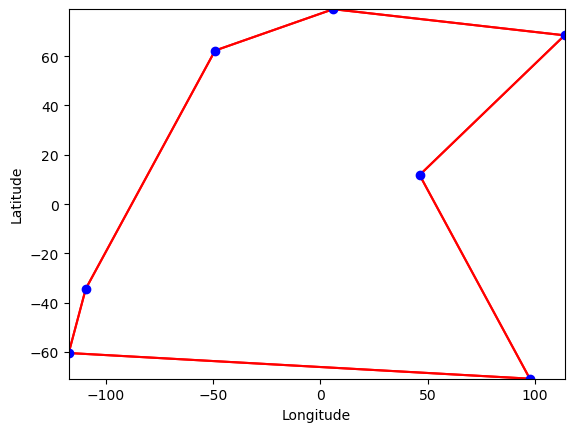
\includegraphics[width=0.3\textwidth]{assets/tsp7.png}
    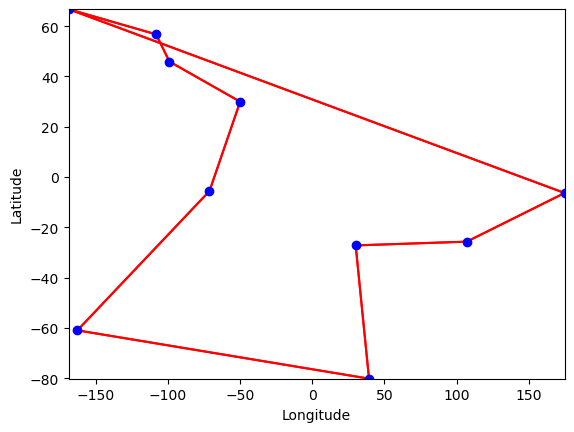
\includegraphics[width=0.3\textwidth]{assets/tsp-10.png}
    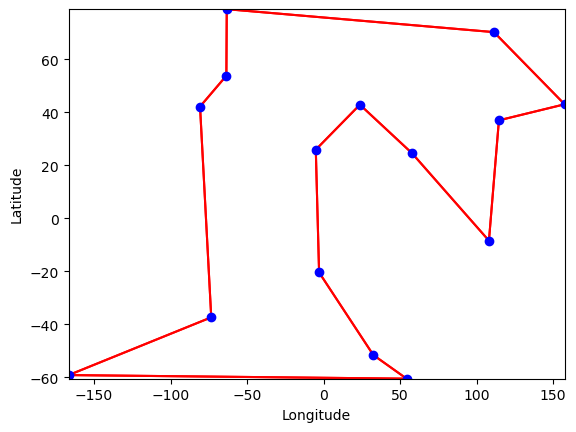
\includegraphics[width=0.3\textwidth]{assets/tsp-15-works.png}
    \caption{reasonable solution}
    \label{fig:TSP Graph}
\end{figure}
\begin{figure}[!ht]
    \centering
    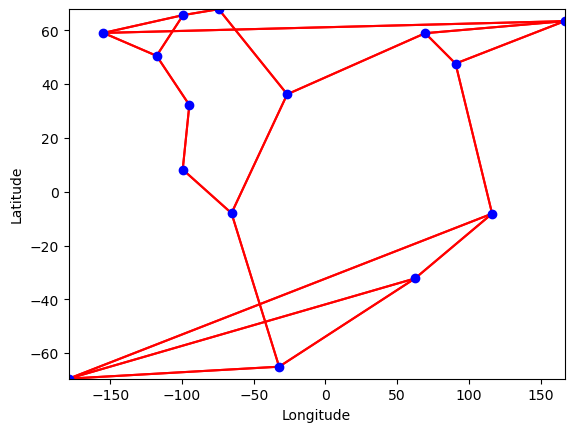
\includegraphics[width=0.3\textwidth]{assets/tsp-15.png}
    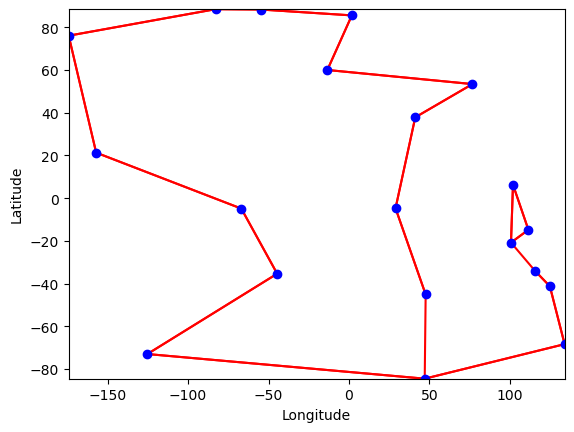
\includegraphics[width=0.3\textwidth]{assets/tsp-20.png}
    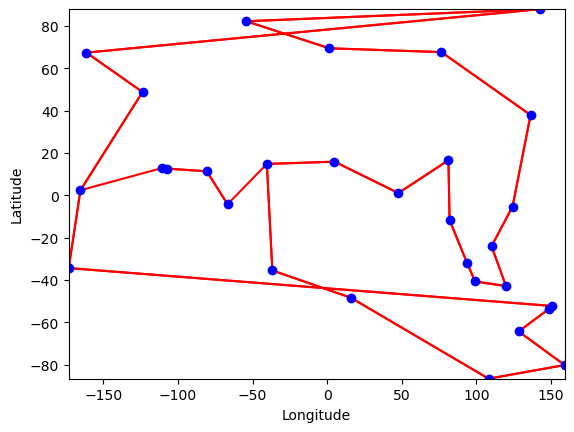
\includegraphics[width=0.3\textwidth]{assets/tsp-30.png}
    \caption{unreasonable solution}
    \label{fig:TSP Graph 2}
\end{figure}


We find that it is easy to break the Hamiltonian cycle, espically as the the number of nodes increases.
\end{frame}
%----------------------------------------------------------------------------------------
%	Matrix Completetion
%----------------------------------------------------------------------------------------

\section{Matrix Completetion} % Sections are added in order to organize your presentation into discrete blocks, all sections and subsections are automatically output to the table of contents as an overview of the talk but NOT output in the presentation as separate slides

%------------------------------------------------

\subsection{Overview}
%
\begin{frame}
	\frametitle{Low rank matrices}
	\begin{center}
		Given an incomplete matrix, can we recover the missing values?
	\end{center}
	\begin{figure}
		\centering 
		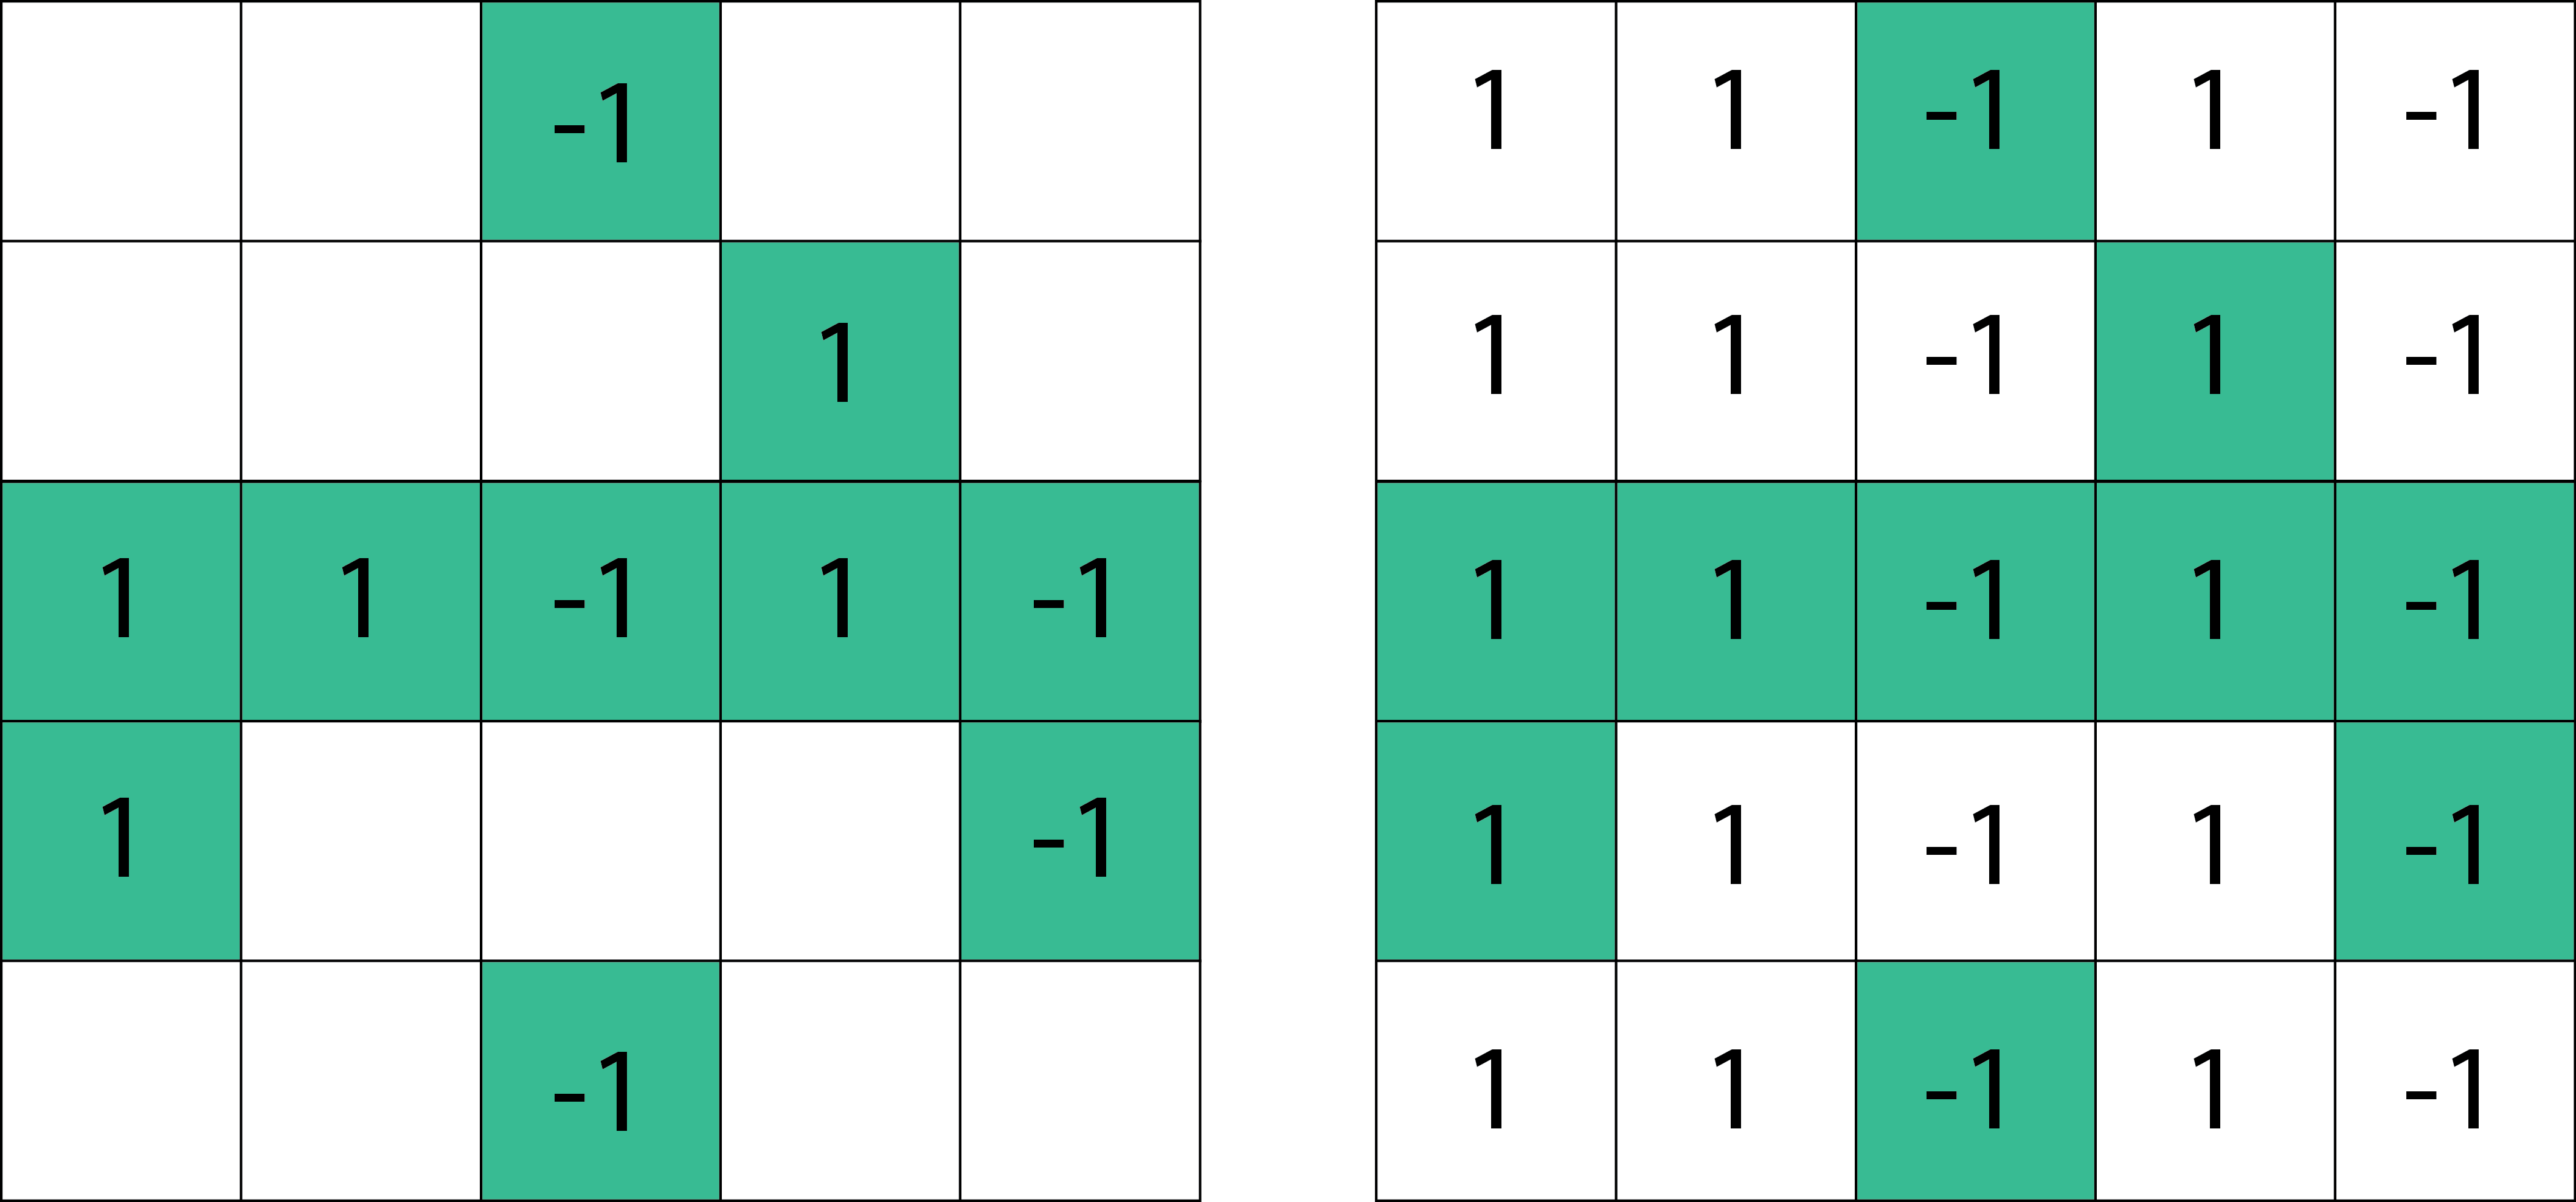
\includegraphics[scale=.3]{assets/mc1.jpg}
		% \caption[]
		% {\tabular[t]{@{}l@{}}Left: a partially filled matrix \\ Right: filling missing values with matrix comple\endtabular}
	\end{figure}
\end{frame}


\begin{frame}
	\frametitle{Low rank matrices}
	\vspace{-5em}
	\begin{center}
		{\huge \textbf{Yes!}}
	\end{center}	
	\vspace{2em}
	Given:
	\begin{itemize}
		\item The matrix is low rank$^*$
		\item We have enough sample data 
		% \item and more ...  (needle in haystack)
	\end{itemize}

	Note: This does not apply to \emph{all} low-rank matrices. But most.
	\vspace{1em}
\end{frame}

\begin{frame}
	\frametitle{Low rank matrices}
	\vspace{-3em}
	\begin{center}
		{\huge \textbf{Yes!}}
	\end{center}	
	\vspace{2em}
	Given:
	\begin{itemize}
		\item The matrix is low rank$^*$
		\item We have enough sample data 
		% \item and more ...  (needle in haystack)
	\end{itemize}

	Note: This does not apply to \emph{all} low-rank matrices. But most.
	\vspace{1em}

	\begin{center}
		\textcolor{blue}{Why low-rank matrices?}		
	\end{center}
\end{frame}

\begin{frame}
	\frametitle{Why is this useful}
	\begin{enumerate}
		\item \textbf{Netflix} has an incomplete set of user preferences based off their past watch history. Can they use this 
		 	   information to recommend new movies?
		\item \textbf{Recommendation Engine:} The netflix problem can be extended to general recommendation engines 
		where a vendor knows some of the user preferences.
		\item \textbf{Images:} We will give an example of recovering a corrupted image using matrix completetion
	\end{enumerate}
\end{frame}

%------------------------------------------------

\subsection{Relaxation} 

\begin{frame}
	\frametitle{Relaxing Matrix Completetion to SDP}
	\vspace{-7em}
	Suppose we have a low rank matrix $\mathbf{M}$. We have a set of location $\Omega$ describing
	our sampling. That is, if $(i,j) \in \Omega$, we observe entry $M_{ij}$. 
	
	Given $\mathbf{M}$ is low rank, 
	it seems resonable that we would like to solve the following optimization problem
	


\end{frame}

\begin{frame}
	\frametitle{Relaxing Matrix Completetion to SDP}
	\vspace{-2.6em}
	Suppose we have a low rank matrix $\mathbf{M}$. We have a set of location $\Omega$ describing
	our sampling. That is, if $(i,j) \in \Omega$, we observe entry $M_{ij}$. 
	
	Given $\mathbf{M}$ is low rank, 
	it seems resonable that we would like to solve the following optimization problem
	
	\begin{equation*}
	  \begin{aligned}
	  & {\text{minimize}}
	  & & \text{rank}(\mathbf{X}) \\[1pt]
	  & \text{subject to}
	  & & X_{ij} = M_{ij} \quad (i,j) \in \Omega\\[1pt]
	  &&& \mathbf{X} \in \mathbb{R}^{n \times n}
	  \end{aligned}
	\end{equation*}

\end{frame}

\begin{frame}
	\frametitle{Relaxing Matrix Completetion to SDP}
	Suppose we have a low rank matrix $\mathbf{M}$. We have a set of location $\Omega$ describing
	our sampling. That is, if $(i,j) \in \Omega$, we observe entry $M_{ij}$. 
	
	Given $\mathbf{M}$ is low rank, 
	it seems resonable that we would like to solve the following optimization problem
	
	\begin{equation*}
	  \begin{aligned}
	  & {\text{minimize}}
	  & & \text{rank}(\mathbf{X}) \\[1pt]
	  & \text{subject to}
	  & & X_{ij} = M_{ij} \quad (i,j) \in \Omega\\[1pt]
	  &&& \mathbf{X} \in \mathbb{R}^{n \times n}
	  \end{aligned}
	\end{equation*}

	\begin{alertblock}{But...}
		Rank is not a convex. This turns out to be an NP-Hard Problem.
	\end{alertblock}
\end{frame}


\begin{frame}
	\frametitle{Introduce the nuclear norm}
	\vspace{-5.5em}
	\begin{block}{Nuclear Norm}
		The nuclear norm is a close approximation of the rank.
	\end{block}
	\vspace{2em}
	
	The nuclear norm of a matrix $\mathbf{X}$ is defined as the sum of 
	the eigenvalues.
	\[
	\lVert \mathbf{X} \rVert_* = \sum_{k=1}^n \sigma_k {\mathbf{X}}  
	\]
\end{frame}

\begin{frame}
	\frametitle{Introduce the nuclear norm}
	\vspace{-4em}
	\begin{block}{Nuclear Norm}
		The nuclear norm is a close approximation of the rank.
	\end{block}
	\vspace{2em}
	
	The nuclear norm of a matrix $\mathbf{X}$ is defined as the sum of 
	the eigenvalues.
	\[
	\lVert \mathbf{X} \rVert_* = \sum_{k=1}^n \sigma_k {\mathbf{X}}  
	\]
	For a symmetric positive semi-definite (SPSD) matricies, the nuclear norm is equal to the trace. 
\end{frame}


\begin{frame}
	\frametitle{A better relaxation}
	What if our matrix is not SPSD
	\begin{itemize}
		\item We introduce two matricies $\mathbf{W}_1$ and $\mathbf{W}_2$ 
	\end{itemize}
\end{frame}

\begin{frame}
	\frametitle{A better relaxation}

	\begin{equation*}
		\begin{aligned}
		& {\text{minimize}}
		& & \text{trace}(\mathbf{W}_1) + \text{trace}(\mathbf{W}_2) \\[1pt]
		& \text{subject to}
		& & X_{ij} = M_{ij} \quad (i,j) \in \Omega\\[1pt]
		&&& \begin{bmatrix} 
		  \mathbf{W}_1 & \mathbf{X} \\
		  \mathbf{X}^\top & \mathbf{W}_2
		\end{bmatrix} \succeq 0 
		\end{aligned}
	  \end{equation*}	
\end{frame}

%------------------------------------------------
\subsection{Fashion-MNIST} 

\begin{frame}
	\frametitle{Fashion-MNIST}
	$55 \%$ of data
	\begin{figure}
		\centering
		
\includegraphics[scale=.3]{assets/mc_ex1_masked.jpeg}
	\end{figure}
\end{frame}

\begin{frame}
	\frametitle{Fashion-MNIST}
	$55 \%$ of data
	\begin{figure}
		\centering
		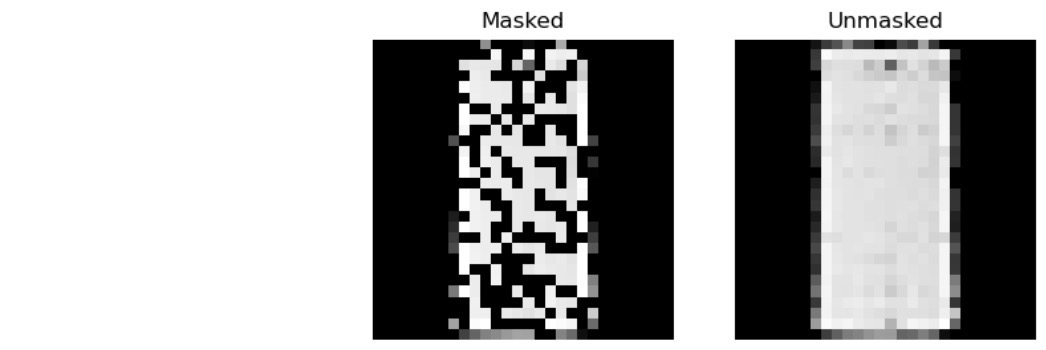
\includegraphics[scale=.3]{assets/mc_ex1_unmasked.jpeg}
	\end{figure}
\end{frame}

\begin{frame}
	\frametitle{Fashion-MNIST}
	$55 \%$ of data
	\begin{figure}
		\centering
		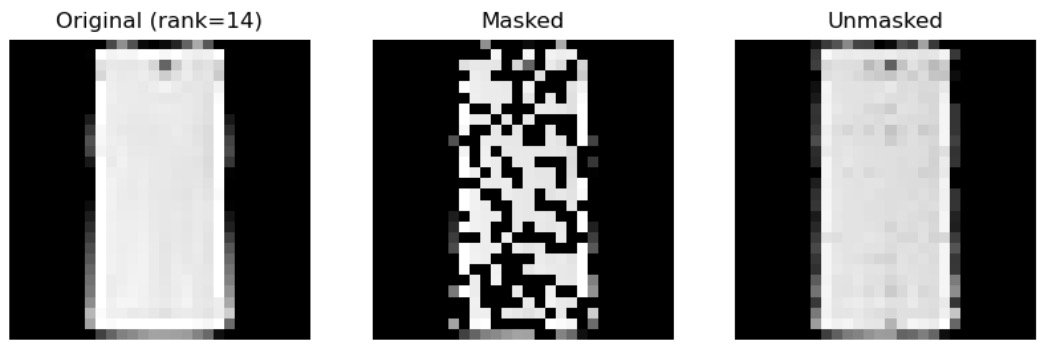
\includegraphics[scale=.3]{assets/mc_ex1_orig.jpg}
	\end{figure}
\end{frame}

\begin{frame}
	\frametitle{Fashion-MNIST}
	$50 \%$ of data
	\begin{figure}
		\centering
		
\includegraphics[scale=.2]{assets/mc_ex2_masked.jpeg}
	\end{figure}
\end{frame}

\begin{frame}
	\frametitle{Fashion-MNIST}
	$50 \%$ of data
	\begin{figure}
		\centering
		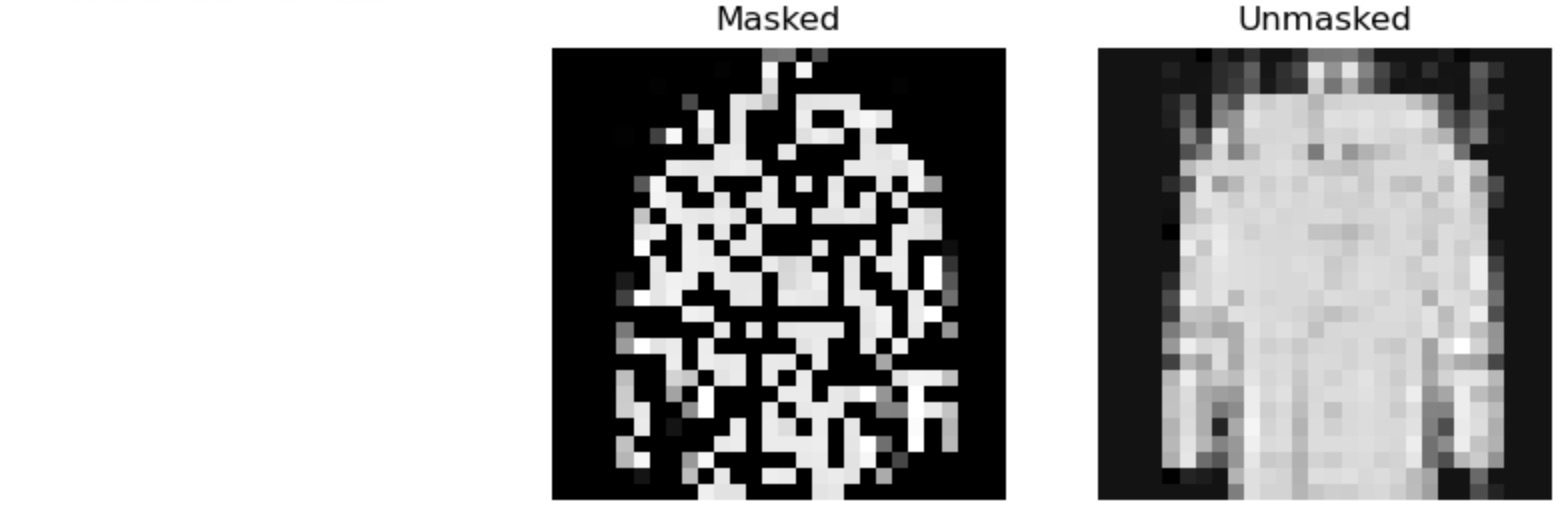
\includegraphics[scale=.2]{assets/mc_ex2_unmasked.jpeg}
	\end{figure}
\end{frame}

\begin{frame}
	\frametitle{Fashion-MNIST}
	$50 \%$ of data
	\begin{figure}
		\centering
		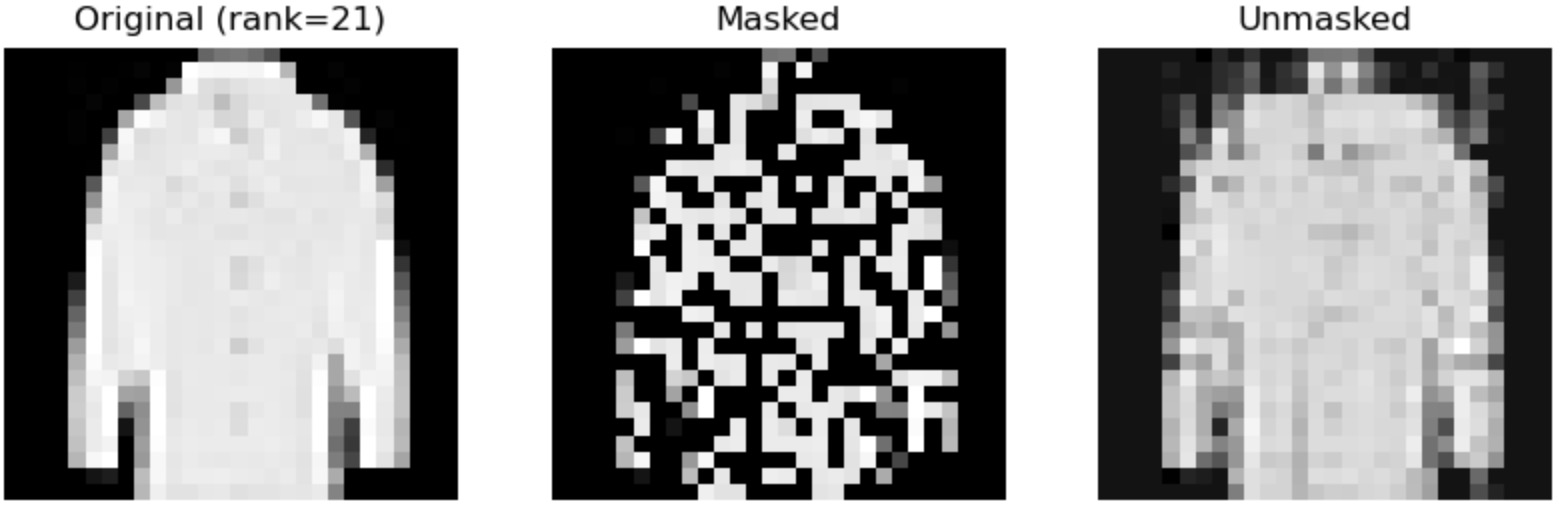
\includegraphics[scale=.2]{assets/mc_ex2_orig.jpg}
	\end{figure}
\end{frame}


%----------------------------------------------------------------------------------------
%	Reference
%----------------------------------------------------------------------------------------

%------------------------------------------------


\section{Referencing}

\begin{frame}
	\frametitle{Citing References}
	
	An example of the \texttt{\textbackslash cite} command to cite within the presentation:
	
	\bigskip % Vertical whitespace
	
	This statement requires citation \cite{p1,p2}.
\end{frame}

%------------------------------------------------

\begin{frame} % Use [allowframebreaks] to allow automatic splitting across slides if the content is too long
	\frametitle{References}
	
	\begin{thebibliography}{99} % Beamer does not support BibTeX so references must be inserted manually as below, you may need to use multiple columns and/or reduce the font size further if you have many references
		\footnotesize % Reduce the font size in the bibliography
		
		\bibitem[Smith, 2022]{p1}
			John Smith (2022)
			\newblock Publication title
			\newblock \emph{Journal Name} 12(3), 45 -- 678.
			
		\bibitem[Kennedy, 2023]{p2}
			Annabelle Kennedy (2023)
			\newblock Publication title
			\newblock \emph{Journal Name} 12(3), 45 -- 678.
	\end{thebibliography}
\end{frame}

%----------------------------------------------------------------------------------------
%	ACKNOWLEDGMENTS SLIDE
%----------------------------------------------------------------------------------------
\begin{frame}
	\frametitle{Acknowledgements}
	
	\begin{columns}[t] % The "c" option specifies centered vertical alignment while the "t" option is used for top vertical alignment
		\begin{column}{0.45\textwidth} % Left column width
			\textbf{Smith Lab}
			\begin{itemize}
				\item Alice Smith
				\item Devon Brown
			\end{itemize}
			\textbf{Cook Lab}
			\begin{itemize}
				\item Margaret
				\item Jennifer
				\item Yuan
			\end{itemize}
		\end{column}		
		\begin{column}{0.5\textwidth} % Right column width
			\textbf{Funding}
			\begin{itemize}
				\item British Royal Navy
				\item Norwegian Government
			\end{itemize}
		\end{column}
	\end{columns}
\end{frame}

\end{document}
